\documentclass[mathserif]{beamer}

\usepackage[english]{babel} % language selection: english/ngerman
                            % note: delete all output files on language change
\usepackage[utf8]{inputenc} % allow for using umlauts
\usepackage{lipsum}         % provide lorem ipsum ...
\usepackage{siunitx}        % provide SI units
\usepackage{amsfonts}       % Provides hollow R for real numbers, hollow C for complex numbers, etc.
\usepackage{algorithm}      % Provides Border for Pseudocode
\usepackage{algpseudocode}  % Provides Pseudocode
\usepackage{interval}       % Provides proper intervals
\usepackage{listings}       % Provides Source Code Listing
\usepackage{gensymb}        % Provides the degree symbol
\usepackage{wrapfig}        % Provides wrapping of text around figures
\usepackage{amssymb}        % Provides empty set symbol (\varnothing)
\usepackage{colortbl}
\usepackage{varwidth}
\usepackage{xcolor}
\usepackage{mathtools}
\usepackage[export]{adjustbox}
\usepackage{subfig}
\usepackage{tikz}
\usepackage{slashbox}
\usepackage{hyperref}
\usepackage{esvect}
\usepackage[makeroom]{cancel}
\usepackage{pdfpages}
\usepackage{amsmath}
\usepackage{outlines}
\usepackage{kbordermatrix}
\usepackage[customcolors]{hf-tikz}
\usepackage{pgfpages}

\usetikzlibrary{arrows.meta}

\tikzset{
    style green/.style={
    set fill color=green!60!lime!40,
    set border color=white,
  },
  style cyan/.style={
    set fill color=cyan!90!blue!60,
    set border color=white,
  },
  style red/.style={
    set fill color=red!30,
    set border color=white,
  },
  style orange/.style={
    set fill color=orange!80!red!40,
    set border color=white,
  },
  hor/.style={
    above left offset={-0.15,0.31},
    below right offset={0.15,-0.10},
    #1
  },
  ver/.style={
    above left offset={-0.10,0.35},
    below right offset={0.10,-0.15},
    #1
  }
}

%\usepackage[T1]{fontenc}
%\usepackage[tt=false,osf]{libertinus}
%\usepackage{inconsolata}

\usetheme[progressbar=frametitle]{metropolis}
%\setbeamertemplate{frame numbering}[fraction]
%\useoutertheme{metropolis}
%\useinnertheme{metropolis}
%\usefonttheme{metropolis}
%\usecolortheme{spruce}
%\setbeamercolor{background canvas}{bg=white}
\metroset{block=fill}

\setbeamertemplate{note page}[plain]
\setbeameroption{show notes on second screen=right}

\title{Gerichtete Graphen}
%\subtitle{Gerichtete Graphen}

\author{Nico Pistel}

\institute[Institute]
{
    Fachbereich Wirtschaft und Informationstechnik\\
    Westfälische Hochschule Bocholt
}

\date{Diskrete Mathematik und Stochastik, 2019}

\subject{Subject}
% This is only inserted into the PDF information catalog. Can be left
% out.

\pgfdeclareimage[height=0.5cm]{university-logo}{img/wh.png}
\logo{\pgfuseimage{university-logo}}

\begin{document}

\begin{frame}
    \titlepage
\end{frame}

\begin{frame}{Outline}
    \tableofcontents
    % You might wish to add the option [pausesections]
\end{frame}

\section{Begriffe \& Definitionen}
\begin{frame}{Begriffe \& Definitionen}
    \begin{outline}
        \1 Ein gerichteter Graph (\textbf{Di}rected \textbf{Graph} - \textit{Digraph}) ist ein Graph, wobei die Kanten mit einer Richtung ausgezeichnet sind\pause
        \1 Unterschied zum ungerichteten Graphen: Kantenrelation $E$ von $G=(V,E)$ ist nicht zwingend symmetrisch\pause
        \2 Adjazenzmatrix $\mathbf{M}$ von $G$ ist nicht zwingend symmetrisch\pause
        \1 Die Richtung der gerichtete Kanten werden durch Pfeile gekennzeichnet\note{Bereits zur Visualisierung von binären Relationen bekannt. Gerichtete Kannten werden auch Arrows, Pfeile oder auch nur Kanten genannt (aus Zusammenhang schließen)}
    \end{outline}
\end{frame}
\begin{frame}{Begriffe \& Definitionen}
    \begin{outline}
        \1 Ein schlichter (Di-)Graph hat keine Schlingen und keine mehrfachen gerichteten Kanten\note{Schlichte (und natürlich ENDLICHE) Digraphen werden betrachtet}\pause
        \1 Anzahl der ausgehenden Kanten von einem Knoten $v$ ist der Ausgangsgrad (\textit{Outdegree}) von $v$: $\deg^+(v)$\pause
        \1 Anzahl der eingehenden Kanten an einem Knoten $v$ ist der Eingangsgrad (\textit{Indegree}) von $v$: $\deg^-(v)$
    \end{outline}\pause
    \begin{lemma}
        \[\sum_{v\in V}\deg^+(v)=\sum_{v\in V}\deg^-(v)=|E|\]
    \end{lemma}
\end{frame}
\begin{frame}{Begriffe \& Definitionen}
    \begin{outline}
        \1 Ein Digraph ist (schwach) zusammenhängend, wenn der zugrunde liegende (ungerichtete) Graph zusammenhängend ist\pause
        \2 Er ist stark zusammenhängend, wenn es zu jeden Knotenpaar $(u,v)$ einen Weg von $u$ nach $v$ gibt und einen Weg von $v$ nach $u$
    \end{outline}
\end{frame}
\begin{frame}{Begriffe \& Definitionen}
    \begin{outline}
        \1 $(u,v)\in E\Longrightarrow$ $u$ ist ein Vorgänger von $v$\pause
        \1 Ein Digraph ohne Zyklen heißt azyklischer Digraph\pause
        \2 \textbf{D}irected \textbf{A}cyclic \textbf{G}raph (\textit{DAG})\pause
        \2 Bei Problemen der Aufgabenplanung heißt ein DAG auch ein PERT-Chart
        \3 Program Evaluation and Review Technique
    \end{outline}
\end{frame}

\section{Topologisches Sortieren}
\begin{frame}{Topologisches Sortieren}
    \begin{outline}
        \1 Beispiel: Aufgaben sollen abgearbeitet werden\pause
        \2 Problem: Aufgaben setzen ggf. voraus, dass andere Aufgaben bereits erledigt wurden\pause
        \2 Motivation: Scheduling, Build-Prozesse\pause
        \1 Problemstellung lässt sich als DAG modellieren\pause
        \2 Warum azyklisch und nicht als allgemeiner (gerichteter) Graph?\pause
        \3 Zyklen deuten auf Aufgaben hin, welche sich selber zur Abarbeitung voraussetzen
        \3 Solche Aufgaben könnten nie abgearbeitet werden
    \end{outline}
\end{frame}
\begin{frame}{Topologisches Sortieren}
    \begin{outline}
        \1 Gesucht ist eine Anordnung, die eine Reihenfolge vorgibt, in welcher die Aufgaben abgearbeitet werden können
        \2 So, dass jede Aufgabe direkt bearbeitet werden kann (alle nötigen Vorausetzungen wurden zuvor erfüllt)\pause
        \1 Eine topologische Sortierung liefert eine solche \textit{konsistente Anordnung} der Knoten\pause
        \1 Für alle Kanten $(u,v)\in E$ gilt, dass $u$ in der Anordnung stets vor $v$ kommt
    \end{outline}
\end{frame}
\begin{frame}{Beispiel: Topologisches Sortieren}
    \centering
    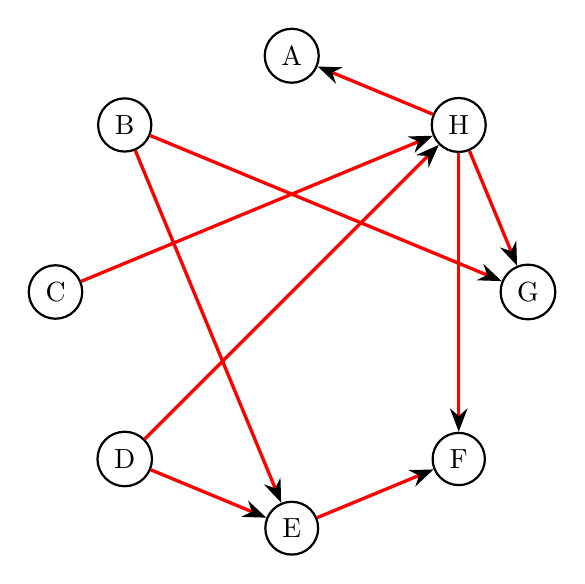
\begin{tikzpicture}
        \begin{scope}[every node/.style={circle,thick,draw}]
            \node (A) at (0 + 3 *  0    , 0 + 3 *  1    ) {A};
            \node (B) at (0 + 3 * -0.707, 0 + 3 *  0.707) {B};
            \node (C) at (0 + 3 * -1    , 0 + 3 *  0    ) {C};
            \node (D) at (0 + 3 * -0.707, 0 + 3 * -0.707) {D};
            \node (E) at (0 + 3 *  0    , 0 + 3 * -1    ) {E};
            \node (F) at (0 + 3 *  0.707, 0 + 3 * -0.707) {F};
            \node (G) at (0 + 3 *  1    , 0 + 3 *  0    ) {G};
            \node (H) at (0 + 3 *  0.707, 0 + 3 *  0.707) {H};
        \end{scope}
        \begin{scope}[>={Stealth[black]}, every edge/.style={draw=red,very thick}]
            \path [->] (B) edge (E);
            \path [->] (B) edge (G);

            \path [->] (C) edge (H);

            \path [->] (D) edge (E);
            \path [->] (D) edge (H);

            \path [->] (E) edge (F);

            \path [->] (H) edge (A);
            \path [->] (H) edge (F);
            \path [->] (H) edge (G);
        \end{scope}
    \end{tikzpicture}
\end{frame}
\begin{frame}{Beispiel: Topologisches Sortieren}
    \centering
    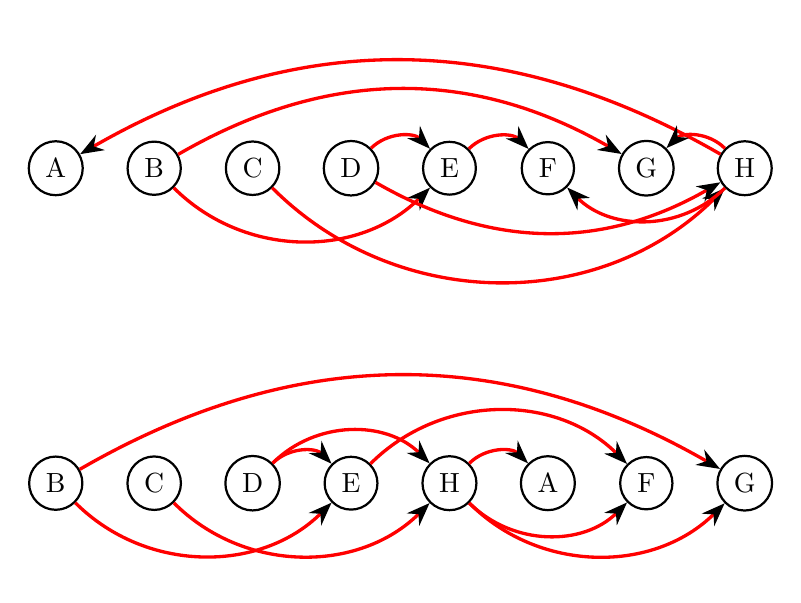
\begin{tikzpicture}
        \begin{scope}[every node/.style={circle,thick,draw}]
            \node (B) at (0.00, -1) {B};
            \node (C) at (1.25, -1) {C};
            \node (D) at (2.50, -1) {D};
            \node (E) at (3.75, -1) {E};
            \node (H) at (5.00, -1) {H};
            \node (A) at (6.25, -1) {A};
            \node (F) at (7.50, -1) {F};
            \node (G) at (8.75, -1) {G};

            \node (Ap) at (0.00, 3) {A};
            \node (Bp) at (1.25, 3) {B};
            \node (Cp) at (2.50, 3) {C};
            \node (Dp) at (3.75, 3) {D};
            \node (Ep) at (5.00, 3) {E};
            \node (Fp) at (6.25, 3) {F};
            \node (Gp) at (7.50, 3) {G};
            \node (Hp) at (8.75, 3) {H};
        \end{scope}
        \begin{scope}[>={Stealth[black]}, every edge/.style={draw=red,very thick}]
            \path [->] (B) edge[bend right=45] (E);
            \path [->] (B) edge[bend right=-30] (G);

            \path [->] (C) edge[bend right=45] (H);

            \path [->] (D) edge[bend right=-45] (E);
            \path [->] (D) edge[bend right=-45] (H);

            \path [->] (E) edge[bend right=-45] (F);

            \path [->] (H) edge[bend right=-45] (A);
            \path [->] (H) edge[bend right=45] (F);
            \path [->] (H) edge[bend right=45] (G);


            \path [->] (Bp) edge[bend right=45] (Ep);
            \path [->] (Bp) edge[bend right=-30] (Gp);

            \path [->] (Cp) edge[bend right=45] (Hp);

            \path [->] (Dp) edge[bend right=-45] (Ep);
            \path [->] (Dp) edge[bend right=30] (Hp);

            \path [->] (Ep) edge[bend right=-45] (Fp);

            \path [->] (Hp) edge[bend right=30] (Ap);
            \path [->] (Hp) edge[bend right=-45] (Fp);
            \path [->] (Hp) edge[bend right=45] (Gp);
        \end{scope}
    \end{tikzpicture}
\end{frame}
\subsection{Kahn's Algorithmus}
\begin{frame}{Kahn's Algorithmus}
    \begin{outline}
        \1 Ein möglicher Algorithmus zur topologischen Sortierung ist Kahn's Algorithmus\pause
        \1 Wechsel der Datenstruktur: Für jeden Knoten $v$ wird die Menge seiner Vorgänger $A(v)$ betrachtet\pause
        \1 Anordnung wird intuitiv erzeugt: In jedem Schritt wird ein Knoten ausgewählt, welcher direkt abgearbeitet werden kann (mögliche Vorgänger sind bereits in der Anordnung vorhanden)\pause
        \1 Wiederholung bis alle Knoten in der Anordnung vorhanden sind\pause
        \1 Es lässt sich immer (mindestens) ein solch ein Knoten auswählen
        \2 Sonst ist ein Zyklus im Graph vorhanden\pause
        \1 Anordnung muss nicht eindeutig sein
        \2 Es können in einem Schritt mehrere Knoten zur Auswahl stehen
    \end{outline}
\end{frame}
\begin{frame}{Beispiel: Kahn's Algorithmus}
    \begin{columns}
        \begin{column}{0.70\textwidth}
            \alt<10->{
                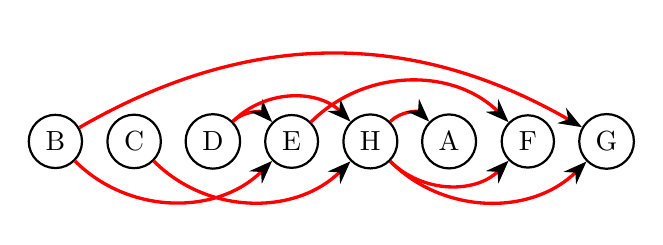
\begin{tikzpicture}
                    \begin{scope}[every node/.style={circle,thick,draw}]
                        \onslide<11->{\node (B) at (0.00, 0) {B};}
                        \onslide<14->{\node (C) at (1.00, 0) {C};}
                        \onslide<17->{\node (D) at (2.00, 0) {D};}
                        \onslide<20->{\node (E) at (3.00, 0) {E};}
                        \onslide<23->{\node (H) at (4.00, 0) {H};}
                        \onslide<26->{\node (A) at (5.00, 0) {A};}
                        \onslide<28->{\node (F) at (6.00, 0) {F};}
                        \onslide<30->{\node (G) at (7.00, 0) {G};}
                    \end{scope}
                    \begin{scope}[>={Stealth[black]}, every edge/.style={draw=red,very thick}]
                        \onslide<20->{\path [->] (B) edge[bend right=45] (E);}
                        \onslide<30->{\path [->] (B) edge[bend right=-30] (G);}

                        \onslide<23->{\path [->] (C) edge[bend right=45] (H);}

                        \onslide<20->{\path [->] (D) edge[bend right=-45] (E);}
                        \onslide<23->{\path [->] (D) edge[bend right=-45] (H);}

                        \onslide<28->{\path [->] (E) edge[bend right=-45] (F);}

                        \onslide<26->{\path [->] (H) edge[bend right=-45] (A);}
                        \onslide<28->{\path [->] (H) edge[bend right=45] (F);}
                        \onslide<30->{\path [->] (H) edge[bend right=45] (G);}
                    \end{scope}
                \end{tikzpicture}
            }{
                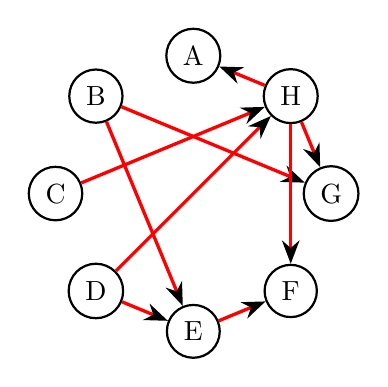
\begin{tikzpicture}
                    \begin{scope}[every node/.style={circle,thick,draw}]
                        \node (A) at (0 + 1.75 *  0    , 0 + 1.75 *  1    ) {A};
                        \node (B) at (0 + 1.75 * -0.707, 0 + 1.75 *  0.707) {B};
                        \node (C) at (0 + 1.75 * -1    , 0 + 1.75 *  0    ) {C};
                        \node (D) at (0 + 1.75 * -0.707, 0 + 1.75 * -0.707) {D};
                        \node (E) at (0 + 1.75 *  0    , 0 + 1.75 * -1    ) {E};
                        \node (F) at (0 + 1.75 *  0.707, 0 + 1.75 * -0.707) {F};
                        \node (G) at (0 + 1.75 *  1    , 0 + 1.75 *  0    ) {G};
                        \node (H) at (0 + 1.75 *  0.707, 0 + 1.75 *  0.707) {H};
                    \end{scope}
                    \begin{scope}[>={Stealth[black]}, every edge/.style={draw=red,very thick}]
                        \path [->] (B) edge (E);
                        \path [->] (B) edge (G);

                        \path [->] (C) edge (H);

                        \path [->] (D) edge (E);
                        \path [->] (D) edge (H);

                        \path [->] (E) edge (F);

                        \path [->] (H) edge (A);
                        \path [->] (H) edge (F);
                        \path [->] (H) edge (G);
                    \end{scope}
                \end{tikzpicture}
            }
        \end{column}
        \begin{column}{0.30\textwidth}
            \begin{tabular}{c|c|c}
                $i$ & $v$ & $A(v)$ \\
                \hline
                \onslide<25>{\tikzmarkin[ver=style green]{r6}}\onslide<26->{$6$} & A & \onslide<2->{$\{\alt<24->{\cancel{\text{H}}}{\text{H}}\}$}\onslide<25>{\tikzmarkend{r6}} \\
                \onslide<10-11>{\tikzmarkin[ver=style green]{r1}}\onslide<11->{$1$} & B & \onslide<3->{$\varnothing$}\onslide<10-11>{\tikzmarkend{r1}} \\
                \onslide<13-14>{\tikzmarkin[ver=style green]{r2}}\onslide<14->{$2$} & C & \onslide<4->{$\varnothing$}\onslide<13-14>{\tikzmarkend{r2}} \\
                \onslide<16-17>{\tikzmarkin[ver=style green]{r3}}\onslide<17->{$3$} & D & \onslide<5->{$\varnothing$}\onslide<16-17>{\tikzmarkend{r3}} \\
                \onslide<19-20>{\tikzmarkin[ver=style green]{r4}}\onslide<20->{$4$} & E & \onslide<6->{$\{\alt<12->{\cancel{\text{B}}}{\text{B}},\alt<18->{\cancel{\text{D}}}{\text{D}}\}$}\onslide<19-20>{\tikzmarkend{r4}} \\
                \onslide<27>{\tikzmarkin[ver=style green]{r7}}\onslide<28->{$7$} & F & \onslide<7->{$\{\alt<21->{\cancel{\text{E}}}{\text{E}},\alt<24->{\cancel{\text{H}}}{\text{H}}\}$}\onslide<27>{\tikzmarkend{r7}} \\
                \onslide<29>{\tikzmarkin[ver=style green]{r8}}\onslide<30->{$8$} & G & \onslide<8->{$\{\alt<12->{\cancel{\text{B}}}{\text{B}},\alt<24->{\cancel{\text{H}}}{\text{H}}\}$}\onslide<29>{\tikzmarkend{r8}} \\
                \onslide<22-23>{\tikzmarkin[ver=style green]{r5}}\onslide<23->{$5$} & H & \onslide<9->{$\{\alt<15->{\cancel{\text{C}}}{\text{C}},\alt<18->{\cancel{\text{D}}}{\text{D}}\}$}\onslide<22-23>{\tikzmarkend{r5}} \\
            \end{tabular}
        \end{column}
    \end{columns}
\end{frame}
\section{Wege in Digraphen}
\begin{frame}{Wege in Digraphen}
    \begin{itemize}
        \item Existenz von Wegen zwischen beliebigen Knoten\pause
        \item Adjazenzmatrix $\mathbf{M}\longrightarrow$ Erreichbarkeitsmatrix $\mathbf{M}^*$\pause
        \item Kantenrelation $E\longrightarrow$ transitiver Abschluss $E^*$
    \end{itemize}
\end{frame}
\subsection{Wege als transitiver Abschluss der Kantenrelation}
\begin{frame}{Wege als transitiver Abschluss der Kantenrelation}
    \begin{itemize}
        \item Kantenrelation $E$: Menge von Wegen der Länge $1$ zwischen Knoten\pause
        \item Menge von Wegen der Länge $2$ als Komposition von $E$ mit sich selber:\\$E\circ E=\{(v_1,v_2)\in V^2|\exists u\in V:(v_1,u)\in E\land(u,v_2)\in E\}$\pause
        \item Menge von Wegen einer Länge $k$: $\underbrace{E\circ\dots\circ E}_{k\text{ mal}}$\note{Nicht Path sondern Walk!}\pause
        \item Transitiver Abschluss als Vereinigung dieser Mengen:\\$E^*=E\cup E\circ E\cup\dots\cup\underbrace{E\circ\dots\circ E}_{\alt<5->{n}{\text{?}}\text{ mal}}$
    \end{itemize}
\end{frame}
\begin{frame}{Potenzieren der Adjazenzmatrix}
    \begin{outline}
        \1 Komposition von $E$ als logisches Matrixprodukt der Adjazenzmatrix $\mathbf{M}$\pause
        \1 Weitere Komposition durch das Potenzieren von $\mathbf{M}$\pause
        \1 Vereinigen der Mengen durch das logische \textbf{oder} der Matrizen
        \1 Logisches \textbf{oder} zweier Matrizen wird komponentenweise gebildet
        \2 $(\mathbf{A}\lor\mathbf{B})_{ij}=\mathbf{A}_{ij}\lor\mathbf{B}_{ij}$
    \end{outline}
    \pause
    \begin{block}{Berechnung der Erreichbarkeitsmatrix $\mathbf{M}^*$}
        \[\mathbf{M}^*=\mathbf{M}\lor\mathbf{M}^2\lor\dots\lor\mathbf{M}^n\]
    \end{block}
\end{frame}
\begin{frame}{Beispiel: Potenzieren der Adjazenzmatrix}
    \begin{columns}
        \begin{column}[t]{0.25\textwidth}
            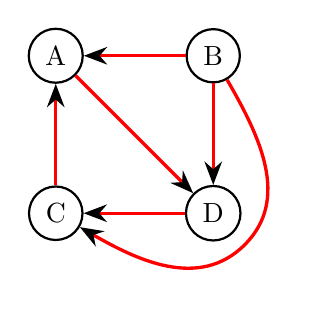
\begin{tikzpicture}
                \begin{scope}[every node/.style={circle,thick,draw}]
                    \node (A) at (0,2) {A};
                    \node (B) at (2,2) {B};
                    \node (C) at (0,0) {C};
                    \node (D) at (2,0) {D};
                \end{scope}
                \begin{scope}[>={Stealth[black]}, every edge/.style={draw=red,very thick}]
                    \path [->] (A) edge (D);
                    \path [->] (B) edge (A);
                    \path [->] (B) edge (D);
                    \path [->] (C) edge (A);
                    \path [->] (D) edge (C);
                    \draw [very thick,draw=red,->] (B) to[out=-60,in=45] (2.40,-0.40) to[out=-135,in=-30] (C);
                \end{scope}
            \end{tikzpicture}
        \end{column}
        \begin{column}{0.70\textwidth}
            \small
            \begin{align*}
                \mathbf{M}&=\kbordermatrix{
                               & \text{A} & \text{B} & \text{C} & \text{D} \\
                      \text{A} &        0 &        0 &        0 &        1 \\
                      \text{B} &        1 &        0 &        1 &        1 \\
                      \text{C} &        1 &        0 &        0 &        0 \\
                      \text{D} &        0 &        0 &        1 &        0
                }
                &\mathbf{M}^2&=\kbordermatrix{
                               & \text{A} & \text{B} & \text{C} & \text{D} \\
                      \text{A} &        0 &        0 &        1 &        0 \\
                      \text{B} &        1 &        0 &        1 &        1 \\
                      \text{C} &        0 &        0 &        0 &        1 \\
                      \text{D} &        1 &        0 &        0 &        0
                }\\
                \mathbf{M}^3&=\kbordermatrix{
                               & \text{A} & \text{B} & \text{C} & \text{D} \\
                      \text{A} &        1 &        0 &        0 &        0 \\
                      \text{B} &        1 &        0 &        1 &        1 \\
                      \text{C} &        0 &        0 &        1 &        0 \\
                      \text{D} &        0 &        0 &        0 &        1
                }
                &\mathbf{M}^4&=\kbordermatrix{
                               & \text{A} & \text{B} & \text{C} & \text{D} \\
                      \text{A} &        0 &        0 &        0 &        1 \\
                      \text{B} &        1 &        0 &        1 &        1 \\
                      \text{C} &        1 &        0 &        0 &        0 \\
                      \text{D} &        0 &        0 &        1 &        0
                }
            \end{align*}
            \[\mathbf{M}^*=\kbordermatrix{
                         & \text{A} & \text{B} & \text{C} & \text{D} \\
                \text{A} &        1 &        0 &        1 &        1 \\
                \text{B} &        1 &        0 &        1 &        1 \\
                \text{C} &        1 &        0 &        1 &        1 \\
                \text{D} &        1 &        0 &        1 &        1
            }\]
        \end{column}
    \end{columns}
\end{frame}
\subsection{Warshall's Algorithmus}
\begin{frame}{Warshall's Algorithmus}
    \begin{outline}
        \pause
        \1 Matrixmultiplikation ist aufwändig
        \2 Berechnen der Potenzen bei Graphen mit vielen Knoten ist problematisch\pause
        \1 Warshall ermittelt $\mathbf{M}^*$ in Worst-Case $\Theta(n^3)$ Zeit
        \1 Warshall's Algorithmus arbeitet \textit{In-Place}
        \2 $\mathbf{M}$ wird iterativ in $\mathbf{M}^*$ überführt\pause
        \1 Warshall erzeugt Matrizen $\mathbf{W}_0,\mathbf{W}_1,\dots,\mathbf{W}_n$
        \2 Wobei $\mathbf{W}_0=\mathbf{M}$ und $\mathbf{W}_n=\mathbf{M}^*$
        \1 $\mathbf{W}_k[i,j]=1\Longleftrightarrow$ Es existiert ein Weg von $v_i$ nach $v_j$, wobei alle Zwischenknoten $\in\{v_1,v_2,\dots,v_k\}$ sind
    \end{outline}
\end{frame}
\begin{frame}{Pseudocode: Warshall's Algorithmus}
    \begin{algorithm}[H]
        \caption{Warshall's Algorithmus}
        \begin{algorithmic}[1]
            \Function{Warshall}{$M$}
                \State $W\gets M$
                \For{$k=1\textbf{ to }n$}
                    \For{$i=1\textbf{ to }n$}
                        \If{$W[i,k]$}
                            \For{$j=1\textbf{ to }n$}
                                \State $W[i,j]\gets W[i,j]\lor W[k,j]$
                            \EndFor
                        \EndIf
                    \EndFor
                \EndFor
                \State \Return $W$
            \EndFunction
        \end{algorithmic}
    \end{algorithm}
\end{frame}
\begin{frame}{Beispiel: Warshall's Algorithmus}
    \begin{columns}
        \begin{column}[t]{0.25\textwidth}
            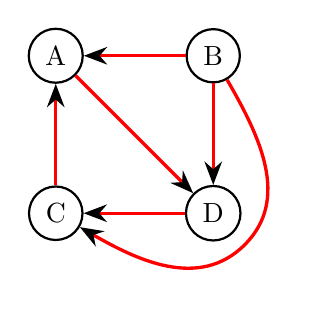
\begin{tikzpicture}
                \begin{scope}[every node/.style={circle,thick,draw}]
                    \node (A) at (0,2) {A};
                    \node (B) at (2,2) {B};
                    \node (C) at (0,0) {C};
                    \node (D) at (2,0) {D};
                \end{scope}
                \begin{scope}[>={Stealth[black]}, every edge/.style={draw=red,very thick}]
                    \path [->] (A) edge (D);
                    \path [->] (B) edge (A);
                    \path [->] (B) edge (D);
                    \path [->] (C) edge (A);
                    \path [->] (D) edge (C);
                    \draw [very thick,draw=red,->] (B) to[out=-60,in=45] (2.40,-0.40) to[out=-135,in=-30] (C);
                \end{scope}
            \end{tikzpicture}
        \end{column}
        \begin{column}{0.70\textwidth}
            \small
            \begin{align*}
                \mathbf{W}_0&=\kbordermatrix{
                               & \text{A} & \text{B} & \text{C} & \text{D} \\
                      \text{A} & \onslide<2-3>{\tikzmarkin[ver=style red]{col 1}}\onslide<4-7>{\tikzmarkin[hor=style red]{row 1}}0 & 0 & 0 & 1\onslide<4-7>{\tikzmarkend{row 1}} \\
                      \text{B} & \onslide<4-5>{\tikzmarkin[hor=style green]{row 2}}1 & 0 & 1 & 1\onslide<4-5>{\tikzmarkend{row 2}} \\
                      \text{C} & \onslide<6-7>{\tikzmarkin[hor=style green]{row 3}}1 & 0 & 0 & 0\onslide<6-7>{\tikzmarkend{row 3}} \\
                      \text{D} & 0\onslide<2-3>{\tikzmarkend{col 1}} & 0 & 1 & 0
                }
                &\mathbf{W}_1&=\kbordermatrix{
                               & \text{A} & \text{B} & \text{C} & \text{D} \\
                      \text{A} & \onslide<3->{0} & \onslide<9-10>{\tikzmarkin[ver=style red]{col 2}}\onslide<3->{0} & \onslide<3->{0} & \onslide<3->{1} \\
                      \text{B} & \onslide<4>{\tikzmarkin[hor=style green]{row 4}}\onslide<5->{1} & \onslide<5->{0} & \onslide<5->{1} & \onslide<5->{1}\onslide<4>{\tikzmarkend{row 4}} \\
                      \text{C} & \onslide<6>{\tikzmarkin[hor=style green]{row 5}}\onslide<7->{1} & \onslide<7->{0} & \onslide<7->{0} & \onslide<7->{1}\onslide<6>{\tikzmarkend{row 5}} \\
                      \text{D} & \onslide<3->{0} & \onslide<3->{0}\onslide<9-10>{\tikzmarkend{col 2}} & \onslide<3->{1} & \onslide<3->{0}
                }\\
                \mathbf{W}_2&=\kbordermatrix{
                               & \text{A} & \text{B} & \text{C} & \text{D} \\
                      \text{A} & \onslide<10->{0} & \onslide<10->{0} & \onslide<12-13>{\tikzmarkin[ver=style red]{col 3}}\onslide<10->{0} & \onslide<10->{1} \\
                      \text{B} & \onslide<14-15>{\tikzmarkin[hor=style green]{row 7}}\onslide<10->{1} & \onslide<10->{0} & \onslide<10->{1} & \onslide<10->{1}\onslide<14-15>{\tikzmarkend{row 7}} \\
                      \text{C} & \onslide<14-17>{\tikzmarkin[hor=style red]{row 6}}\onslide<10->{1} & \onslide<10->{0} & \onslide<10->{0} & \onslide<10->{1}\onslide<14-17>{\tikzmarkend{row 6}} \\
                      \text{D} & \onslide<16-17>{\tikzmarkin[hor=style green]{row 8}}\onslide<10->{0} & \onslide<10->{0} & \onslide<10->{1}\onslide<12-13>{\tikzmarkend{col 3}} & \onslide<10->{0}\onslide<16-17>{\tikzmarkend{row 8}}
                }
                &\mathbf{W}_3&=\kbordermatrix{
                               & \text{A} & \text{B} & \text{C} & \text{D} \\
                      \text{A} & \onslide<20-21>{\tikzmarkin[hor=style green]{row 12}}\onslide<13->{0} & \onslide<13->{0} & \onslide<13->{0} & \onslide<19>{\tikzmarkin[ver=style red]{col 4}}\onslide<13->{1}\onslide<20-21>{\tikzmarkend{row 12}} \\
                      \text{B} & \onslide<22-23>{\tikzmarkin[hor=style green]{row 13}}\onslide<14>{\tikzmarkin[hor=style green]{row 9}}\onslide<15->{1} & \onslide<15->{0} & \onslide<15->{1} & \onslide<15->{1}\onslide<14>{\tikzmarkend{row 9}}\onslide<22-23>{\tikzmarkend{row 13}} \\
                      \text{C} & \onslide<24-25>{\tikzmarkin[hor=style green]{row 14}}\onslide<13->{1} & \onslide<13->{0} & \onslide<13->{0} & \onslide<13->{1}\onslide<24-25>{\tikzmarkend{row 14}} \\
                      \text{D} & \onslide<26-27>{\tikzmarkin[hor=style orange]{row 19}}\onslide<20-25>{\tikzmarkin[hor=style red]{row 11}}\onslide<16>{\tikzmarkin[hor=style green]{row 10}}\onslide<17->{1} & \onslide<17->{0} & \onslide<17->{1} & \onslide<17->{1}\onslide<16>{\tikzmarkend{row 10}}\onslide<19>{\tikzmarkend{col 4}}\onslide<20-25>{\tikzmarkend{row 11}}\onslide<26-27>{\tikzmarkend{row 19}}
                }
            \end{align*}
            \[\mathbf{W}_4=\kbordermatrix{
                         & \text{A} & \text{B} & \text{C} & \text{D} \\
                \text{A} & \onslide<20>{\tikzmarkin[hor=style green]{row 15}}\onslide<21->{1 & 0 & 1 & 1}\onslide<20>{\tikzmarkend{row 15}} \\
                \text{B} & \onslide<22>{\tikzmarkin[hor=style green]{row 16}}\onslide<23->{1 & 0 & 1 & 1}\onslide<22>{\tikzmarkend{row 16}} \\
                \text{C} & \onslide<24>{\tikzmarkin[hor=style green]{row 17}}\onslide<25->{1 & 0 & 1 & 1}\onslide<24>{\tikzmarkend{row 17}} \\
                \text{D} & \onslide<26>{\tikzmarkin[hor=style green]{row 18}}\onslide<27-28>{1 & 0 & 1 & 1}\onslide<26>{\tikzmarkend{row 18}}
            }\]
        \end{column}
    \end{columns}
\end{frame}
\section{Kürzeste Wege}
\begin{frame}{Kürzeste Wege}
    \begin{outline}
        \1 Gewichteter Digraph: Jede Kante bekommt ein reelle Zahl zugeordnet
        \2 Gewicht, Kosten, Distanz, \dots dieser Kante\pause
        \1 Auffindung von Wegen minimaler Gesamtdistanz\pause
        \1 Motivation: Routingprotokolle (OSPF), Routenplanung, Basis für Suchalgorithmen aus der künstlichen Intelligenz\pause
        \1 Gewichteter Digraph lässt sich durch Gewichtsmatrix $\mathbf{W}$ repräsentieren, wobei\[\mathbf{W}_{ij}=\begin{cases}0,&i=j\\\infty,&(v_i,v_j)\notin E\\d(v_i,v_j),&sonst\end{cases}\]
    \end{outline}
\end{frame}
\subsection{Dijkstra's Algorithmus}
\begin{frame}{Dijkstra's Algorithmus}
    \pause
    \begin{outline}
        \1 Dijkstra's Algorithmus löst das \textit{Single-Source Shortest-Path Problem}\pause
        \2 Findet zu einem gegebenen Startknoten einen kürzesten Weg zu jedem anderen Knoten des Digraphen\pause
        \2 Eine Modifikation des Algorithmus von Warshall (Floyd-Warshall-Algorithmus) löst das \textit{All-Nodes Shortest-Path Problem}\pause
        \1 Vorausetzung für Dijkstra's Algorithmus sind nicht negative Kantengewichte für alle Kanten\pause
        \2 Ein alternativer Algorithmus (Bellman-Ford-Algorithmus) löst das Problem auch für negative Kantengewichte (jedoch generell langsamer)\pause
        \2 Gilt jedoch nur, sofern keine negative Zyklen (Zyklen mit negativem Gesamtgewicht) existieren
        \3 Sonst gibt es keinen eindeutigen Shortest-Path
    \end{outline}
\end{frame}
\begin{frame}{Dijkstra's Algorithmus}
    \begin{outline}
        \1 Dijkstra betrachtet im Algorithmus die (aktuelle) Distanz $d(v)$ eines Knotens $v$ vom Startknoten $A$\pause
        \1 Trivialerweise ist $d(A)=0$, alle anderen Knoten bekommen zunächst eine Distanz von $\infty$ zugewiesen (sind also noch nicht erreichbar)\pause
        \1 In jedem Schritt des Algorithmus wird ein Knoten betrachtet, abgearbeitet und \textit{markiert}
        \2 Markierte Knoten gelten als abgearbeitet und werden nicht weiter betrachtet oder verändert
    \end{outline}
\end{frame}
\begin{frame}{Dijkstra's Algorithmus}
    \begin{outline}
        \1 Es wird stets der von $A$ am nächsten liegende Knoten $u$ (welcher nicht markiert ist) ausgewählt und markiert\pause
        \1 Von diesem Knoten aus werden alle benachbarte Knoten $v$ (welche nicht markiert sind) betrachtet\pause
        \2 Es wird die Distanz von $A$ nach $v$ als $d(u)+d(u,v)$ berechnet (die Distanz von $A$ nach $u$ und von $u$ nach $v$)
        \2 Ist diese Summe kleiner als die aktuelle Distanz von $A$ nach $v$, wird $d(v)$ mit der zuvor berechneten Summe aktualisiert\pause
        \1 Dies wird solange wiederholt, bis alle Knoten einmal betrachtet (und markiert) wurden
    \end{outline}
\end{frame}
\begin{frame}{Dijkstra's Algorithmus}
    \begin{outline}
        \1 Um später auch den kürzesten Weg von $A$ zu einem beliebigen Knoten $v$ rekonstruieren zu können, wird üblicherweise auch ein \textit{Parent}-Attribut $p(v)$ mitgeführt
        \2 Dieses enthält den Vorgänger von $v$ im aktuell kürzesten Weg von $A$ nach $v$
        \2 Dieses Feld wird im Laufe des Algorithmus zusammen mit $d(v)$ aktualisiert
    \end{outline}
\end{frame}
\begin{frame}[t]{Beispiel: Dijkstra's Algorithmus}
    \begin{columns}
        \begin{column}{0.70\textwidth}
            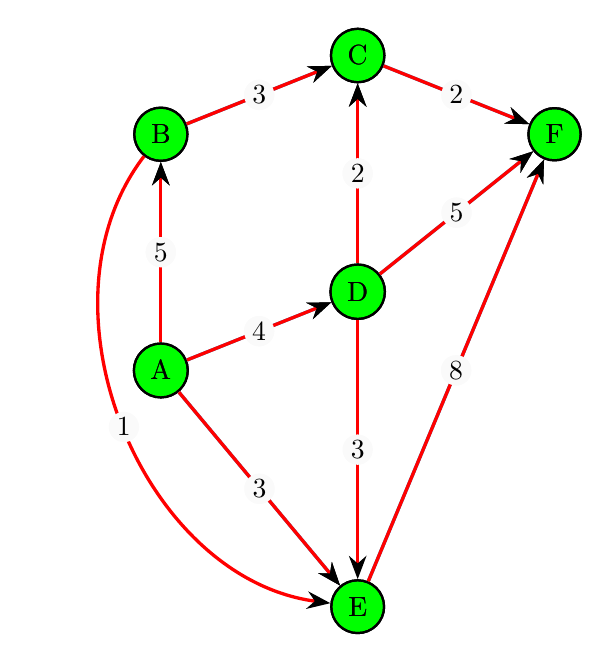
\begin{tikzpicture}
                \begin{scope}[every node/.style={circle,thick,draw}]
                    \alt<4->{\node[fill=green] (A) at (0,0) {A};}{\node (A) at (0,0) {A};}
                    \alt<15->{\node[fill=green] (B) at (0,3) {B};}{\node (B) at (0,3) {B};}
                    \alt<18->{\node[fill=green] (C) at (2.5,4) {C};}{\node (C) at (2.5,4) {C};}
                    \alt<10->{\node[fill=green] (D) at (2.5,1) {D};}{\node (D) at (2.5,1) {D};}
                    \alt<7->{\node[fill=green] (E) at (2.5,-3) {E};}{\node (E) at (2.5,-3) {E};}
                    \alt<21->{\node[fill=green] (F) at (5,3) {F};}{\node (F) at (5,3) {F};}
                \end{scope}

                \begin{scope}[>={Stealth[black]},every node/.style={inner sep=1pt,fill={rgb,255:red,250;green,250;blue,250},circle},every edge/.style={draw=red,very thick}]
                    \alt<5>{\path [->] (A) edge[draw=cyan] node {$5$} (B);}{\path [->] (A) edge node {$5$} (B);}
                    \alt<16>{\path [->] (B) edge[draw=cyan] node {$3$} (C);}{\path [->] (B) edge node {$3$} (C);}
                    \alt<5>{\path [->] (A) edge[draw=cyan] node {$4$} (D);}{\path [->] (A) edge node {$4$} (D);}
                    \alt<11>{\path [->] (D) edge[draw=cyan] node {$2$} (C);}{\path [->] (D) edge node {$2$} (C);}
                    \alt<5>{\path [->] (A) edge[draw=cyan] node {$3$} (E);}{\path [->] (A) edge node {$3$} (E);}
                    \path [->] (D) edge node {$3$} (E);
                    \alt<13>{\path [->] (D) edge[draw=cyan] node {$5$} (F);}{\path [->] (D) edge node {$5$} (F);}
                    \alt<19>{\path [->] (C) edge[draw=cyan] node {$2$} (F);}{\path [->] (C) edge node {$2$} (F);}
                    \alt<8>{\path [->] (E) edge[draw=cyan] node {$8$} (F);}{\path [->] (E) edge node {$8$} (F);}
                    \path [->] (B) edge[bend right=60] node {$1$} (E);
                \end{scope}
            \end{tikzpicture}
        \end{column}
        \begin{column}{0.30\textwidth}
            \begin{tabular}{c|c|c}
                $v$ & $d(v)$ & $p(v)$ \\
                \hline
                \onslide<4->{\tikzmarkin[hor=style green]{n1}}A & \onslide<2->{$0$} & \onslide<2->{$\varnothing$}\onslide<4->{\tikzmarkend{n1}} \\
                \onslide<15->{\tikzmarkin[hor=style green]{n10}}\onslide<6>{\tikzmarkin[hor=style red]{n2}}B & \onslide<3->{\alt<6->{$5$}{$\infty$}} & \onslide<3->{\alt<6->{A}{$\varnothing$}}\onslide<6>{\tikzmarkend{n2}}\onslide<15->{\tikzmarkend{n10}} \\
                \onslide<18->{\tikzmarkin[hor=style green]{n11}}\onslide<12>{\tikzmarkin[hor=style red]{n8}}C & \onslide<3->{\alt<12->{$6$}{$\infty$}} & \onslide<3->{\alt<12->{D}{$\varnothing$}}\onslide<12>{\tikzmarkend{n8}}\onslide<18->{\tikzmarkend{n11}} \\
                \onslide<10->{\tikzmarkin[hor=style green]{n7}}\onslide<6>{\tikzmarkin[hor=style red]{n3}}D & \onslide<3->{\alt<6->{$4$}{$\infty$}} & \onslide<3->{\alt<6->{A}{$\varnothing$}}\onslide<6>{\tikzmarkend{n3}}\onslide<10->{\tikzmarkend{n7}} \\
                \onslide<7->{\tikzmarkin[hor=style green]{n5}}\onslide<6>{\tikzmarkin[hor=style red]{n4}}E & \onslide<3->{\alt<6->{$3$}{$\infty$}} & \onslide<3->{\alt<6->{A}{$\varnothing$}}\onslide<6>{\tikzmarkend{n4}}\onslide<7->{\tikzmarkend{n5}} \\
                \onslide<21->{\tikzmarkin[hor=style green]{n13}}\onslide<20>{\tikzmarkin[hor=style red]{n12}}\onslide<14>{\tikzmarkin[hor=style red]{n9}}\onslide<9>{\tikzmarkin[hor=style red]{n6}}F & \onslide<3->{\alt<20->{$8$}{\alt<14->{$9$}{\alt<9->{$11$}{$\infty$}}}} & \onslide<3->{\alt<20->{C}{\alt<14->{D}{\alt<9->{E}{$\varnothing$}}}}\onslide<9>{\tikzmarkend{n6}}\onslide<14>{\tikzmarkend{n9}}\onslide<20>{\tikzmarkend{n12}}\onslide<21->{\tikzmarkend{n13}}
            \end{tabular}
        \end{column}
    \end{columns}
\end{frame}
\begin{frame}[t]{Shortest-Path Baum}
    \begin{columns}
        \begin{column}{0.70\textwidth}
            \onslide<2->{
                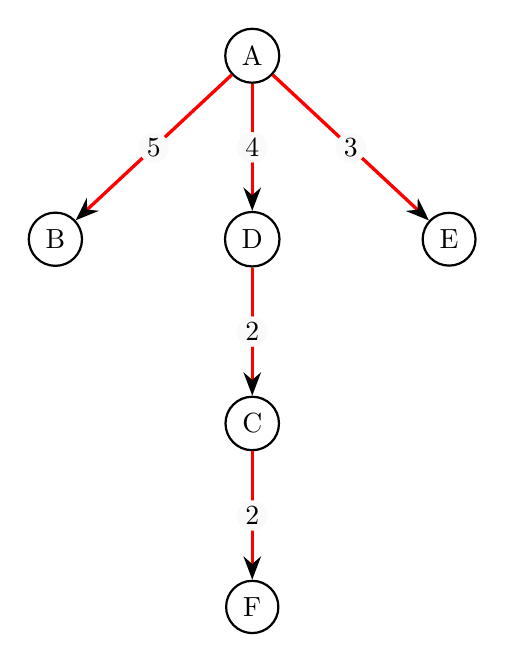
\begin{tikzpicture}
                    \begin{scope}[every node/.style={circle,thick,draw}]
                        \node (A) at (2.5, 4) {A};
    
                        \node (B) at (0, 1.67) {B};
                        \node (D) at (2.5, 1.67) {D};
                        \node (E) at (5, 1.67) {E};
    
                        \node (C) at (2.5,-0.67) {C};
    
                        \node (F) at (2.5,-3) {F};
                    \end{scope}
                    \begin{scope}[>={Stealth[black]},every node/.style={inner sep=1pt,fill={rgb,255:red,250;green,250;blue,250},circle},every edge/.style={draw=red,very thick}]
                        \path [->] (A) edge node {$5$} (B);
                        \path [->] (A) edge node {$4$} (D);
                        \path [->] (D) edge node {$2$} (C);
                        \path [->] (A) edge node {$3$} (E);
                        \path [->] (C) edge node {$2$} (F);
                    \end{scope}
                \end{tikzpicture}
            }
        \end{column}
        \begin{column}{0.30\textwidth}
            \begin{tabular}{c|c|c}
                $v$ & $d(v)$ & $p(v)$ \\
                \hline
                A & $0$ & $\varnothing$ \\
                B & $5$ & A \\
                C & $6$ & D \\
                D & $4$ & A \\
                E & $3$ & A \\
                F & $8$ & C \\
            \end{tabular}
        \end{column}
    \end{columns}
\end{frame}

\end{document}